\documentclass[11pt,a4paper]{article}
\usepackage[margin=2cm]{geometry}
\usepackage{graphicx}
\usepackage{xcolor}
\usepackage{tcolorbox}
\usepackage{enumitem}
\usepackage{multicol}
\usepackage{amsmath}
\usepackage{amssymb}
\usepackage{fancyhdr}
\usepackage{hyperref}
\usepackage{tikz}
\usetikzlibrary{arrows.meta, positioning, shapes}

% Define colors
\definecolor{mlblue}{RGB}{31, 119, 180}
\definecolor{mlorange}{RGB}{255, 127, 14}
\definecolor{mlgreen}{RGB}{44, 160, 44}
\definecolor{mlred}{RGB}{214, 39, 40}
\definecolor{mlpurple}{RGB}{148, 103, 189}

% Header and footer
\pagestyle{fancy}
\fancyhf{}
\lhead{Week 1: Clustering \& Innovation}
\rhead{Post-Class Theory Synthesis}
\cfoot{Page \thepage}

\title{\Large\textbf{From Discovery to Theory:\\Clustering \& Innovation Synthesis}\\
\vspace{0.5em}
\large Post-Class Handout - Week 1}
\author{BSc Machine Learning for Innovation\\
\textit{Theory Building from Your Discoveries}}
\date{}

\begin{document}
\maketitle
\thispagestyle{fancy}

\begin{tcolorbox}[colback=mlgreen!10, colframe=mlgreen!50, title={\textbf{Connecting Your Discoveries to Theory}}]
In the pre-class session, you discovered patterns and created rules. Now we'll connect your insights to formal clustering theory and see how they drive innovation in real organizations.
\end{tcolorbox}

\section*{Part 1: Your Discoveries Have Names!}

\subsection*{The Dot Cloud Mystery - What You Found}

Remember when you identified groups in the dot cloud? Here's what you actually discovered:

\begin{multicols}{2}
\textbf{Your Observation:}
\begin{itemize}
\item ``Dots near each other belong together''
\item ``Groups have empty space between them''
\item ``Some dots are between groups''
\end{itemize}

\columnbreak

\textbf{The Theory Names:}
\begin{itemize}
\item \textcolor{mlblue}{Proximity} (Distance-based clustering)
\item \textcolor{mlorange}{Separation} (Inter-cluster distance)
\item \textcolor{mlred}{Outliers} (Boundary points)
\end{itemize}
\end{multicols}

\begin{tcolorbox}[colback=mlblue!10, colframe=mlblue!50, title={\textbf{Theory Connection: Clustering}}]
\textbf{Clustering} = Finding natural groups in data without labels\\
Your rule-making exercise was actually \textit{unsupervised learning} - discovering structure without being told the answer!
\end{tcolorbox}

\subsection*{Innovation Application}

\begin{center}
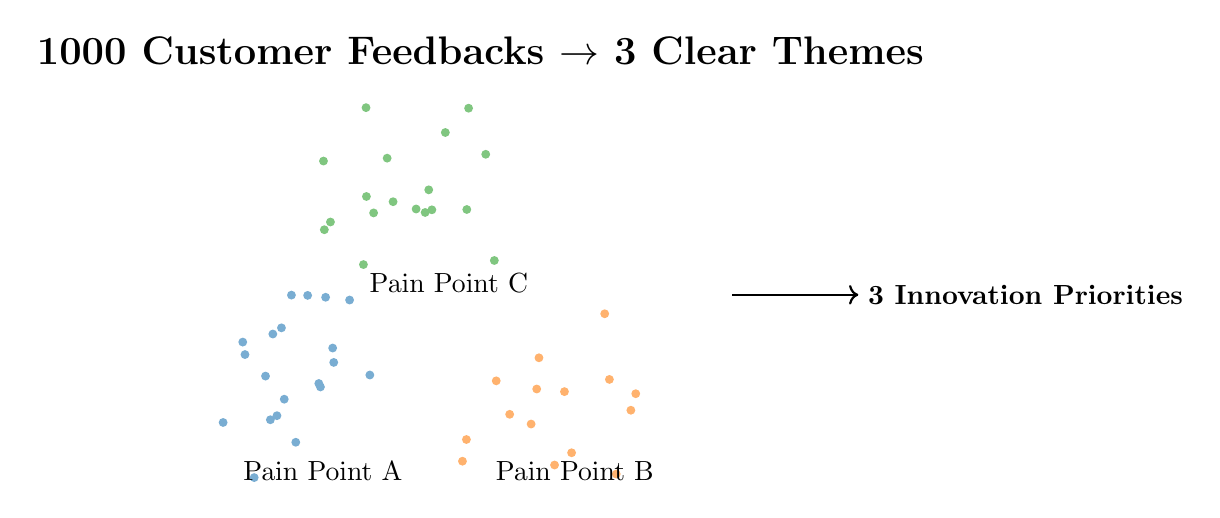
\begin{tikzpicture}[scale=0.8]
% Customer feedback points
\foreach \i in {1,...,20}
    \fill[mlblue!60] (rand*1.5+1, rand*1.5+1) circle (2pt);
\foreach \i in {1,...,15}
    \fill[mlorange!60] (rand*1.5+5, rand*1.5+1) circle (2pt);
\foreach \i in {1,...,18}
    \fill[mlgreen!60] (rand*1.5+3, rand*1.5+4) circle (2pt);

% Labels
\node[below] at (1.5, 0) {Pain Point A};
\node[below] at (5.5, 0) {Pain Point B};
\node[below] at (3.5, 3) {Pain Point C};

% Arrow to innovation
\draw[->, thick] (8, 2.5) -- (10, 2.5);
\node[right] at (10, 2.5) {\textbf{3 Innovation Priorities}};

\node[above] at (4, 6) {\Large\textbf{1000 Customer Feedbacks $\rightarrow$ 3 Clear Themes}};
\end{tikzpicture}
\end{center}

\newpage
\section*{Part 2: The Distance Concept - Your Rules Formalized}

\subsection*{Your Similarity Rules Become Distance Metrics}

When you grouped the 5 students, you created a \textbf{distance metric}:

\begin{tcolorbox}[colback=white, colframe=mlpurple!50]
\textbf{Your Rule} (Example): ``Similar if tech skills are close AND creativity is close''\\
\textbf{Mathematical Form}: $d = \sqrt{(tech_1 - tech_2)^2 + (creativity_1 - creativity_2)^2}$\\
\textbf{Theory Name}: \textcolor{mlpurple}{Euclidean Distance}
\end{tcolorbox}

\subsection*{Different Rules = Different Algorithms}

\begin{center}
\includegraphics[width=\textwidth]{visual6_algorithm_grid.pdf}
\end{center}

\begin{multicols}{2}
\textbf{K-means} (Your ``average'' rule):
\begin{itemize}
\item Finds center points
\item Creates circular groups
\item Good for similar-sized groups
\end{itemize}

\columnbreak

\textbf{DBSCAN} (Your ``density'' rule):
\begin{itemize}
\item Finds dense regions
\item Any shape groups
\item Identifies outliers
\end{itemize}
\end{multicols}

\section*{Part 3: The Innovation Journey - Your Process Map}

Remember the mystery panels (1000 → ? → ? → 5)? Here's what happens:

\begin{center}
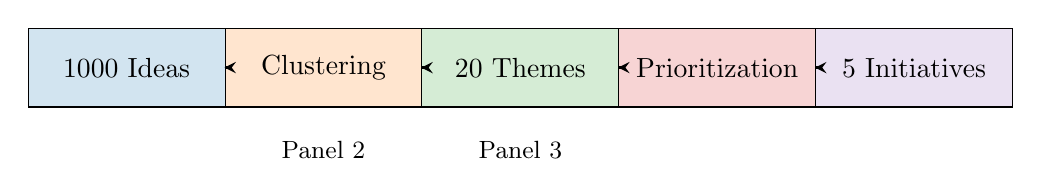
\begin{tikzpicture}[node distance=2.5cm]
\tikzstyle{process} = [rectangle, minimum width=2.5cm, minimum height=1cm, text centered, draw=black, fill=mlblue!20]
\tikzstyle{arrow} = [thick,->,>=stealth]

\node (input) [process] {1000 Ideas};
\node (cluster) [process, right of=input, fill=mlorange!20] {Clustering};
\node (themes) [process, right of=cluster, fill=mlgreen!20] {20 Themes};
\node (prioritize) [process, right of=themes, fill=mlred!20] {Prioritization};
\node (output) [process, right of=prioritize, fill=mlpurple!20] {5 Initiatives};

\draw [arrow] (input) -- (cluster);
\draw [arrow] (cluster) -- (themes);
\draw [arrow] (themes) -- (prioritize);
\draw [arrow] (prioritize) -- (output);

\node[below=0.3cm of cluster] {\small Panel 2};
\node[below=0.3cm of themes] {\small Panel 3};
\end{tikzpicture}
\end{center}

\begin{tcolorbox}[colback=mlorange!10, colframe=mlorange!50, title={\textbf{The Mathematical Pattern You Found}}]
\textbf{Complexity Reduction}: $\sqrt{n}$ rule\\
1000 → $\sqrt{1000} \approx 32$ → filter → 5\\
500 → $\sqrt{500} \approx 22$ → filter → 3\\
This is \textit{dimensionality reduction} - making complex problems manageable!
\end{tcolorbox}

\newpage
\section*{Part 4: Building Your Personal Framework}

\subsection*{From Theory Seeds to Full Concepts}

Connect your discoveries to the formal definitions:

\begin{center}
\begin{tabular}{|l|l|p{6cm}|}
\hline
\textbf{Theory Seed} & \textbf{Your Discovery} & \textbf{Formal Definition} \\
\hline
Proximity & Dots close together & Intra-cluster distance minimization \\
\hline
Similarity & Same characteristics & Feature space distance \\
\hline
Homogeneity & Groups look alike inside & Low within-cluster variance \\
\hline
Separation & Space between groups & High between-cluster variance \\
\hline
Cohesion & Groups stick together & Cluster compactness measure \\
\hline
Distinction & Groups are different & Cluster separability \\
\hline
\end{tabular}
\end{center}

\subsection*{Your Innovation Toolkit}

Based on your discoveries, you now have tools for:

\begin{multicols}{2}
\textbf{Finding Opportunities:}
\begin{itemize}
\item Look for clustering in problems
\item Identify white spaces (no clusters)
\item Find overlapping themes
\end{itemize}

\columnbreak

\textbf{Creating Solutions:}
\begin{itemize}
\item Group similar ideas
\item Prioritize by cluster size
\item Target specific segments
\end{itemize}
\end{multicols}

\section*{Part 5: Practice Challenge}

\subsection*{Real Innovation Scenario}

You have 500 product reviews. Use your clustering knowledge to:

\begin{enumerate}
\item \textbf{Define your distance metric}: What makes reviews ``similar''?
\begin{tcolorbox}[colback=white, colframe=gray!50, height=2cm]
\vspace{1.5cm}
\end{tcolorbox}

\item \textbf{Choose your algorithm}: K-means, DBSCAN, or Hierarchical? Why?
\begin{tcolorbox}[colback=white, colframe=gray!50, height=2cm]
\vspace{1.5cm}
\end{tcolorbox}

\item \textbf{Decide cluster count}: How many product themes do you expect?
\begin{tcolorbox}[colback=white, colframe=gray!50, height=2cm]
\vspace{1.5cm}
\end{tcolorbox}

\item \textbf{Innovation action}: What would you do with the clusters?
\begin{tcolorbox}[colback=white, colframe=gray!50, height=2cm]
\vspace{1.5cm}
\end{tcolorbox}
\end{enumerate}

\newpage
\section*{Part 6: Key Takeaways}

\begin{tcolorbox}[colback=mlgreen!10, colframe=mlgreen!50, title={\textbf{What You've Discovered \& Learned}}]
\begin{itemize}
\item \textbf{Clustering is pattern finding} - You did this naturally with dots
\item \textbf{Distance defines similarity} - Your rules determine the groups
\item \textbf{Different algorithms for different patterns} - Shape matters
\item \textbf{Innovation needs structure} - 1000 ideas → 20 themes → 5 actions
\item \textbf{You can find opportunities} - White spaces between clusters
\end{itemize}
\end{tcolorbox}

\subsection*{The Innovation Equation}

\begin{center}
\Large
\begin{tcolorbox}[colback=mlblue!10, colframe=mlblue!70, width=0.8\textwidth]
\centering
\textbf{Many Ideas} + \textbf{Clustering} + \textbf{Human Insight} = \textbf{Strategic Innovation}
\end{tcolorbox}
\end{center}

\subsection*{Your Next Steps}

\begin{enumerate}
\item \textbf{In Class}: We'll implement K-means together
\item \textbf{Practice}: Apply clustering to your project domain
\item \textbf{Think}: Where else could grouping reveal insights?
\end{enumerate}

\begin{tcolorbox}[colback=mlpurple!10, colframe=mlpurple!50, title={\textbf{Reflection Questions}}]
\begin{itemize}
\item Which clustering approach fits your innovation challenge?
\item How would you explain clustering to a non-technical teammate?
\item What patterns might be hiding in your organization's data?
\end{itemize}
\end{tcolorbox}

\vspace{1cm}

\begin{tcolorbox}[colback=gray!10, colframe=gray!50, title={\textbf{Mathematical Deep Dive (Optional)}}]
\small
\textbf{K-means Objective Function}: $J = \sum_{i=1}^{n} \sum_{j=1}^{k} w_{ij} ||x_i - \mu_j||^2$

\textbf{Silhouette Score}: $s(i) = \frac{b(i) - a(i)}{\max\{a(i), b(i)\}}$

Where $a(i)$ is average intra-cluster distance and $b(i)$ is average nearest-cluster distance.

\textbf{Want more?} See the main lecture appendix for complete mathematical foundations.
\end{tcolorbox}

\end{document}